%%%%%%%%%%%%%%%%%%%%%%%%%%%%%%%%%%%%%%%%%%%%%%%%%%%%%%%
%%      TCC de Lucas Rodrigues de Carvalho, 2016     %%
%%%%%%%%%%%%%%%%%%%%%%%%%%%%%%%%%%%%%%%%%%%%%%%%%%%%%%%

% Alterado por Prof. Fernando C.B.G. Santana
% A simplificação visa melhorar a navegação e edição

%% Preâmbulo (configurações, pacotes e tudo mais)

\documentclass[
	%article,			% Define que este será um artigo (e não uma tese/monografia/relatório)
	12pt,				% Fonte: 12pt
	oneside,			% Impressão: oneside = 1 face, twoside = 2 faces (frente-e-verso)
    %openright,			% capítulos começam em página ímpar (use apenas se usar "twoside")
	a4paper,			% Tamanho do Papel: A4
    chapter=TITLE,		% Todos os capítulos devem ficam em caixa alta
    section=TITLE,		% Todas as seções devem ficar em caixa alta
	english,			% Adiciona Idioma para Hifenização: Inglês
    %spanish,			% Adiciona Idioma para Hifenização: Espanhol
    %french,			% Adiciona Idioma para Hifenização: Francês
	brazil				% Adiciona Idioma para Hifenização: Português do Brasil (o último idioma se torna o principal do documento)
]{abntex2}				% Utilizar ABNTeX2

%% Tipografia
%% Abra este arquivo e selecione uma das opções de fonte nele. A padrão é Times.
%% Tipografia / Fontes
%% AVISO: Todas essas fontes são *bastante semelhantes* aos nomes com as quais as descrevo. Entenda: são iguais, só que oficialmente com outro nome.

%% %%%%%%%%%%%%%%%%%%%%%%%%%%%%%%%%%%%%%%%%%%%%%%%%%%%%% %%
%% Comente todas as outras fontes que você não vai usar! %%
%% %%%%%%%%%%%%%%%%%%%%%%%%%%%%%%%%%%%%%%%%%%%%%%%%%%%%% %%

%% Latin Modern (fonte padrão do LaTeX, Computer Modern, mas com suporte a caracteres acentuados)
%% Considerada a mais clássica e bonita
%\usepackage{lmodern}



%% Times
%% Considerada a mais confortável de ler quando impresso
\usepackage{mathptmx}

%% Variação da mesma fonte, com minúsculas diferenças entre uma e outra (coisas bastante técnicas como kerning, aliasing e afins) - Essa tem revisões frequentes
%\usepackage{newtxtext} \usepackage{newtxmath}



%% Arial
%% Considerada mais confortável de ler num computador
%% ** Oficialmente recomendada pelo manual de formatação do IFPI **
%\usepackage{helvet} \renewcommand{\familydefault}{\sfdefault}



%% Palatino
%% Uma opção mais elegante à Times
%\usepackage{newpxtext}



%% Kepler
%% Variação evoluída da Palatino, com várias pequenas diferenças e refinamentos
%\usepackage{kpfonts}



%% Libertine
%% Uma fonte estilo Serif comum no Linux
%\usepackage{libertine} %\usepackage[libertine]{newtxmath}

%% Pacotes usados pelo documento (se não entender não mexa, hehehe)
\usepackage{courier}                    % Permite a utilização da fonte Courier (para códigos-fonte)
\usepackage[T1]{fontenc}				% Seleção de códigos de fonte.
\usepackage[utf8]{inputenc}				% Codificação do documento (conversão automática dos acentos)
\usepackage{indentfirst}				% Indenta o primeiro parágrafo de cada seção.
\usepackage{nomencl} 					% Usado pela Lista de símbolos
\usepackage{color}						% Controle das cores
\usepackage{graphicx}					% Inclusão de gráficos
\let\newfloat\undefined
\usepackage{float}						% Melhorias para posicionamento de gráficos e tabelas
\usepackage{microtype} 					% Melhorias na justificação
\usepackage{lastpage}   		        % Dá acesso ao número da última página do documento
\usepackage{booktabs}					% Comandos para tabelas
\usepackage{multirow, array}			% Múltiplas linhas e colunas em tabelas
\usepackage[hyphenbreaks]{breakurl}		% Hifenação para URLs no texto
\usepackage[table,xcdraw]{xcolor}       % Cores para algumas tabelas especiais
\usepackage[brazilian,hyperpageref]{backref}	 % Inclui nas Referências as páginas onde há as citações
\usepackage{simplecd}                   % Pacote para gerar capa do CD
\usepackage[final]{pdfpages}            % Pacote para incluir um PDF dentro de outro (ficha catalográfica)

%% Adiciona as alterações do ABNTeX-IFPI
\usepackage{abntex-ifpi/abntex-ifpi}	% Modificações do ABNTeX para o IFPI
\usepackage{abntex-ifpi/tikz-uml}	    % Pacote Tikz UML para criar UML no LaTeX

%% Metadados
%% Configurações dos metadados do PDF
\makeatletter
\hypersetup{
  pdftitle={\@title}, 
  pdfauthor={\@author},
  pdfsubject={\@title},
  pdfcreator={LaTeX, abnTeX2, {abnTeX\-ifpi}},
  %% Coloque aqui suas palavras-chave, cada uma entre chaves: {palavra}{palavra}{outra palavra}...
  pdfkeywords={financiamento coletivo}{empreendimento social}{crowdfunding}{impacto social}{social impact}{social entrepreneurship},
  colorlinks=true,			% Visual dos Links: false = caixas; true = colorido
  linkcolor=cor-link,		% Cor dos Links Internos (preto)
  citecolor=cor-link,		% Cor de Links para Bibliografia (preto)
  filecolor=cor-link,		% Cor para Links a Arquivos (preto)
  urlcolor=cor-link,		% Cor para Links a URLs (preto)
  bookmarksdepth=4
}
\makeatother
%% Metadados
%% %%%%%%%%%%%%%%%%%%%%%%%%%%%%%%%%%%%%%%%%%%%%%%%% %%
%% Metadados do trabalho
%% AVISO: Todos esses dados serão automaticamente convertidos para caixa alta onde necessário
%% %%%%%%%%%%%%%%%%%%%%%%%%%%%%%%%%%%%%%%%%%%%%%%%% %%

%% Título
\titulo{Protótipo de Aplicativo de Navegação Indoor para o Instituto Federal do Piauí  }

%% Autor
\autor{Maykon da Costa Menezes}

%% Nome do Curso (usado para a Capa do CD)
\nomedocurso{Análise e Desenvolvimento de Sistemas}

%% Local de publicação
\local{Teresina, Piauí}

%% Preâmbulo do trabalho
\preambulo{Projeto apresentado à Banca Examinadora como requisito para aprovação na disciplina de Trabalho de Conclusão de Curso I do Curso Superior de Tecnologia em Análise e Desenvolvimento de Sistemas do Instituto Federal de Educação, Ciência e Tecnologia do Piauí.}

%% Orientador
%% "M\textsuperscript{e}." = Abreviação oficial para "Mestre"
\orientador{ Prof.ª Me. Valéria Oliveira Costa}

%% Tipo de Trabalho
%% - Monografia
%% - Tese (Mestrado)
%% - Tese (Doutorado)
%% - Relatório técnico
\tipotrabalho{Monografia}

%% Data do Trabalho
\data{2019}

%% Nome da Instituição (para a capa)
\instituicao{INSTITUTO FEDERAL DE EDUCAÇÃO, CIÊNCIA E TECNOLOGIA DO PIAUÍ
\\
CAMPUS TERESINA CENTRAL
\\
TECNOLOGIA EM ANÁLISE E DESENVOLVIMENTO DE SISTEMAS}

%% Primeiro membro da banca examinadora
\membroum{Membro 1}

%% Segundo membro da banca examinadora
\membrodois{Membro 2}

%% Terceiro membro da banca examinadora
\membrotres{Membro 3}



%% Data da apresentação do trabalho
%% Se não souber a data da apresentação, utilize \underline{\hspace{3.5cm}}
%% Isso cria um sublinhado de 3.5cm, onde você pode escrever a data depois!
%\dataapresentacao{04 de Abril de 2017}
\dataapresentacao{\underline{\hspace{3.5cm}}}

%% Configuração do "Citado nas páginas"
%% Configuração das Citações

%% Estilo
%\usepackage[num]{abntex2cite}			% Citações numéricas
\usepackage[brazilian,hyperpageref]{backref}     % Paginas com as citações na bibl
\usepackage[alf]{abntex2cite}			% Citações "AUTOR, ano"



%% Colocar entre parênteses ou colchetes?
%% Padrão: Parênteses
%% * Fica mais agradável usar colchetes quando se usa citações numéricas
\citebrackets[]							% Comente essa linha e o documento usará parênteses


%% Configura o "Citado nas Páginas ..." nas referências
%% Não mexa nesse:
\renewcommand{\backref}{}

%% Esse é o texto do "Citado nas páginas ..."
\renewcommand*{\backrefalt}[4]{
	\ifcase #1
		Nenhuma citação no texto.
	\or
		Citado na página #2.
	\else
		Citado #1 vezes nas páginas #2.
	\fi}
%% Cores
%% Cores do Documento

%% Cor dos Links do PDF
%% Usando preta você "esconde" os links
\definecolor{cor-link}{RGB}{0,0,0}

%% Usando azul os links ficam visíveis (ruim para impressão)
%\definecolor{cor-link}{RGB}{8,40,75}



%% Cor para os quadros
%% Dê preferência a cores escuras.
%% Boa referência para cores: https://material.io/guidelines/style/color.html#color-color-palette
\definecolor{cor-quadro}{RGB}{5,28,63}		% Azul Escuro
%% Espaçamentos
%% Espaçamentos
%% O tamanho do parágrafo é dado por:
\setlength{\parindent}{1.3cm}

%% Espaçamento entre um parágrafo e outro:
%% O abntex diz: "tente também \onelineskip"
\setlength{\parskip}{0.2cm}

%% Início do Documento
\begin{document}

%% Documento será escrito em Português do Brasil
\selectlanguage{brazil}

%% Elementos Pré Textuais
%% ----------------------
%% 
%% Segundo o manual do IFPI, eles devem ser os seguintes (nessa ordem):
%%  1. Capa (obrigatório)
%%  2. Folha de rosto (obrigatório)
%%  3. Errata (opcional)
%%  4. Folha de aprovação (obrigatório)
%%  5. Dedicatória (opcional)
%%  6. Agradecimentos (opcional)
%%  7. Epígrafe (opcional)
%%  8. Resumo (obrigatório)
%%  9. Abstract/Resumo em outra língua (obrigatório)
%% 10. Lista de Ilustrações (opcional)
%% 11. Lista de Tabelas (opcional)
%% 12. Lista de Abreviaturas e Siglas (opcional)
%% 13. Lista de Símbolos (opcional)
%% 14. Sumário (obrigatório)
%% %%%%%%%%%%%%%%%%%%%%%%%%%%%%%%%%%%%%%%%%% %%

%% 01: Capa
\imprimircapa

%% 02: Folha de Rosto
%% OBS: O asterisco indica que haverá ficha bibliográfica (só funciona para impressão frente-e-verso)
\imprimirfolhaderosto*

%% Ficha Catalográfica (acho que é melhor adicionar via \includepdf depois)
%%% Ficha Catalográfica
%%
%% Este template cria um quadro semelhante a ficha catalográfica oficial.
%% É melhor usar \includepdf depois que a ficha oficial estiver em mãos.

%% Caso tenha o arquivo PDF da ficha
%% A ficha catalográfica do IFPI pode ser gerada através neste link: https://sistemas.ifpi.edu.br/fichacatalografica/
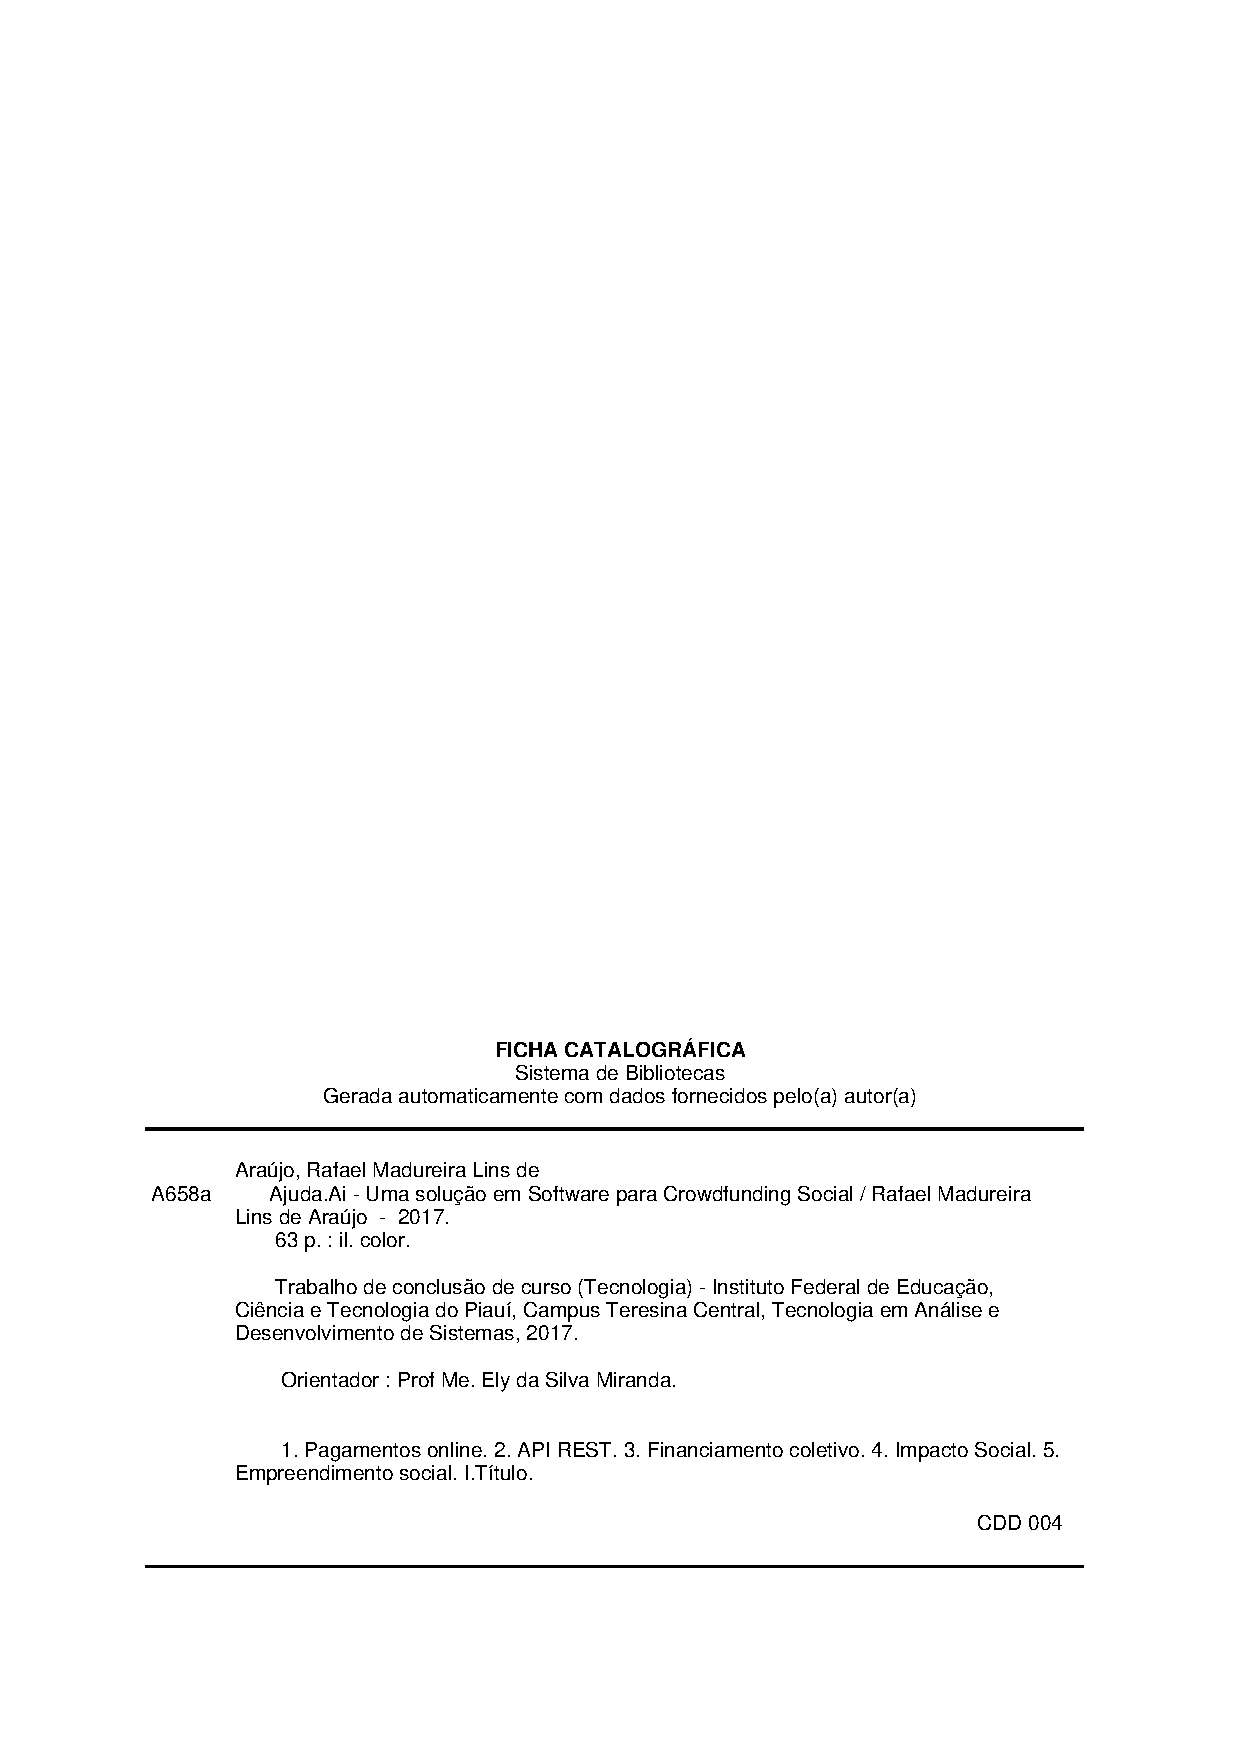
\includepdf{pre-textual/ficha-catalografica.pdf}

%% Caso queira fazer a ficha "tradicional" (este serve apenas como um modelo)
%\begin{fichacatalografica}
%	\sffamily
%	\vspace*{\fill}					% Posição vertical
%	\begin{center}					% Minipage Centralizado
%	\fbox{\begin{minipage}[c][8cm]{13.5cm}		% Largura
%	\small
%	\imprimirautor
%	
%	\hspace{0.5cm} \imprimirtitulo  / \imprimirautor. --
%	\imprimirlocal, \imprimirdata-
%	
%	\hspace{0.5cm} \thelastpage p. : il. (algumas color.) ; 30 cm.\\
%	
%	\hspace{0.5cm} \imprimirorientadorRotulo~\imprimirorientador\\
%	
%	\hspace{0.5cm}
%	\parbox[t]{\textwidth}{\imprimirtipotrabalho~--~\imprimirinstituicao,
%	\imprimirdata.}\\
%	
%	\hspace{0.5cm}
%		1. Palavra-chave1.
%		2. Palavra-chave2.
%		2. Palavra-chave3.
%		I. Orientador.
%		II. Universidade xxx.
%		III. Faculdade de xxx.
%		IV. Título 			
%	\end{minipage}}
%	\end{center}
%\end{fichacatalografica}

%% 03: Errata
%%% Errata
%\begin{errata}
%Elemento opcional da norma ABNT NBR14724 de 2011. Exemplo:
%
%\vspace{\onelineskip}
%
%FERRIGNO, C. R. A. \textbf{Tratamento de neoplasias ósseas apendiculares com reimplantação de enxerto ósseo autólogo autoclavado associado ao plasma rico em plaquetas}: estudo crítico na cirurgia de preservação de membro em cães. 2011. 128 f. Tese (Livre-Docência) - Faculdade de Medicina Veterinária e Zootecnia, Universidade de São Paulo, São Paulo, 2011.

%% Tabela de exemplo com os erros
%\begin{table}[htb]
%\center
%\footnotesize
%\begin{tabular}{|p{1.4cm}|p{1cm}|p{3cm}|p{3cm}|}
%  \hline
%   \textbf{Folha} & \textbf{Linha}  & \textbf{Onde se lê}  & \textbf{Leia-se}  \\
%    \hline
%    1 & 10 & auto-conclavo & autoconclavo\\
%   \hline
%\end{tabular}
%\end{table}
%
%\end{errata}

%% 04: Folha de Aprovação
%\imprimirfolhadeaprovacao
%% Use esta se forem 4 membros na banca:
\imprimirfolhadeaprovacaoduascolunas

%% 05: Dedicatória
%%% Dedicatória do seu trabalho
\begin{dedicatoria}
	%% Empura o texto a seguir para a parte de baixo da página
	\vspace*{\fill}
    
    %% Alinhado a Direita
    \center
    \begin{flushright}
    	Dedicatória.
    \end{flushright}
    
    %% Descomente a linha seguir para deixar o texto centralizado verticalmente na página
    %% Lembre de comentar o "\begin{}" e "\end{}" acima para centralizar o texto da dedicatória.
	%\vspace*{\fill}
\end{dedicatoria}


%% 06: Agradecimentos
%% Agradecimentos
\begin{agradecimentos}
	Agradecimentos
\end{agradecimentos}


%% 07: Epígrafe
%% Epígrafe
%% Uma frase que lhe inspira ou a qual lhe inspirou a fazer este trabalho
\begin{epigrafe}
\vspace*{\fill}
\begin{flushright}
\emph{``Epigrafe'' \\ (Autor)}
\end{flushright}
\end{epigrafe}


%% 08: Resumo
%% Resumo
\begin{resumo}
A demanda por serviços de localização indoor (LBS) vem aumentando ao longo dos anos juntamente com
a expansão do mercado de smartphones. Há um crescente interesse no desenvolvimento de sistemas de navegação indoor para dispositivos móveis. Usuários de smartphones não conseguem navegar em áreas internas utilizando o GPS do aparelho pois ele não consegue fixar a localização exata de acordo com a função do GPS receiver. Essa é a grande razão da gigantesca demanda por informações de localização em tempo real de usuários desses portáteis. A função de GPS receiver tem uma poderosa precisão para localização em ambientes externos, mas em contrapartida o mesmo não se mostra eficaz por causa de atenuação de sinal.

Abordagens com informações pré-existentes sobre o ambiente (campos magnéticos, Bluetooth, WiFi) juntamente com dados de sensores dos smartphones (magnetômetro, giroscópio e acelerômetro) tem atraído mais e mais atenção por serem(.. a completar) . Este trabalho propõe um protótipo de aplicativo android de navegação indoor eficiente que une informações pré-existentes do ambiente com dados de sensores dos smartphones.


\vspace{\onelineskip}
\noindent
\textbf{Palavras-chaves}: Palavras chave.
\end{resumo}


%% 09: Abstract/Resumo em língua estrangeira
%% Abstract (configurado para língua inglesa)
\begin{resumo}[Abstract]			% Título do Resumo (Abstract = Resumo em inglês)
\begin{otherlanguage*}{english}		% Língua do texto
The demand for Indoor Location Based Services
(LBS) is increasing over the past years as
smartphone market expands. There's a growing
interest in developing efficient and reliable
indoor positioning systems for mobile devices.
Smartphone users can get their fixed locations
according to the function of the GPS receiver.
This is the primary reason why there is a huge
demand for real-time location information of
mobile users. However, the GPS receiver is
often not effective in indoor environments due
to signal attenuation, even as the major
positioning devices have a powerful accuracy
for outdoor positioning.

Using preexisting information about the environment(magnetics, bluetooth, WiFi) among with smartphone's sensors data (compass, gyroscope, accelerator) attract more and more attention due to. This paper proposes an efficient and reliable android application prototype of indoor navagation.

\vspace{\onelineskip}
\noindent
\textbf{Key-words}: Palavras-chave em língua estrangeira.
\end{otherlanguage*}
\end{resumo}

%% Exemplo de resumo em francês
%\begin{resumo}[Résumé]
% \begin{otherlanguage*}{french}
%    Il s'agit d'un résumé en français.
% 
%   \textbf{Mots-clés}: latex. abntex. publication de textes.
% \end{otherlanguage*}
%\end{resumo}

%% Exemplo de resumo em Espanhol
%\begin{resumo}[Resumen]
% \begin{otherlanguage*}{spanish}
%   Este es el resumen en español.
%  
%   \textbf{Palabras clave}: latex. abntex. publicación de textos.
% \end{otherlanguage*}
%\end{resumo}
% ---


%% 10: Lista de Ilustrações
%% Lista de Ilustrações
\pdfbookmark[0]{\listfigurename}{lof}
\listoffigures*
\cleardoublepage

%% 11: Lista de Tabelas
%% Lista de Tabelas
%\pdfbookmark[0]{\listtablename}{lot}
%\listoftables*
%\cleardoublepage

%% 12: Lista de Abreviaturas e Siglas
%% Lista de Siglas
\begin{siglas}
  \item[API] Application Programming Interface
  \item[WWW] World Wide Web
  \item[REST] Representational State Transfer
  \item[HTML5] Hypertext Markup Language, versão 5
  \item[JSON] JavaScript Object Notation
  \item[CSS] Cascading Style Sheets
  \item[MVC] Model View Controller
  \item[CDI] Contexts and Dependency Injection
  \item[ORM] Object/Relational Mapping
  \item[JDBC] Java DataBase Connection
  \item[SGBD] Sistema de Gerenciamento de Banco de Dados
  \item[UUID] Universally Unique Identifier
  \item[CRUD] Create, Read, Update e Delete - Operações básicas de o SGBD
\end{siglas}

%% 13: Lista de Símbolos
% %% Lista de Símbolos
%% (esta é apenas uma lista de exemplo)
%\begin{simbolos}
%  \item[$ \Gamma $] Letra grega Gama
%  \item[$ \Lambda $] Lambda
%  \item[$ \zeta $] Letra grega minúscula zeta
%  \item[$ \in $] Pertence
%\end{simbolos}

%% 14: Sumário (o asterisco retira o próprio sumário do sumário)
\pdfbookmark[0]{\contentsname}{toc}
\tableofcontents*
\cleardoublepage

%% Indica que a partir daqui ficarão os elementos textuais (TCC em si)
\textual
%% Inclui os capítulos do TCC
% ----------------------------------------------------------
% Introdução
% ----------------------------------------------------------
\chapter{Introdução}

Com o rápido desenvolvimento da comunicação através de portáteis e a difusão de tecnologias de computação em todas as áreas, a necessidade de se obter serviços de localização e navegação está rapidamente crescendo. Melhorias dramáticas em performance dos padrões de comunicação moveis tem impulsionado a tecnologia móvel a se tornar o meio mais rápido de comunicação de todos os tempos. Os custos de infraestrutura com redes moveis também caíram drasticamente, enquanto performance só tem melhorado.

Na ultima década, temos visto grandes melhorias na redução de tamanho de hardwares, a chegada de muitas novas tecnologias, como redes wireless, baterias com grandes capacidades, chips de alta performance etc, que fazem do smartphone uma ferramenta poderosa. Essas tecnologias permitiram que os fabricantes construíssem dispositivos moveis que podem ser carregados por ai com a mesma performance de computadores tradicionais. Os benefícios de toda essa tecnologia embarcada pode ser aproveitada pelos chamados serviços baseados em localização. Aplicações que guiam usuários, que se comportam diferente baseado na localização ou contexto do usuário, ou melhor, que conseguem navegar o usuário através de um local e oferecer informações baseado em onde ele está são atualmente “trend topic”  em pesquisa e são considerados como um mercado promissor.

Atualmente, o Sistema de Posicionamento Global (GPS) oferece informação de localização precisa e confiável para serviços de localização. O GPS não pode ser usado efetivamente dentro de um ambiente interno porque ocorre uma degradação de sinal. Por outro lado, informações pré-existentes do ambiente e sensores que possibilitam localizar como acelerômetros, giroscópios, magnetômetro, WiFi, câmeras etc podem ser usados por serviços baseados em localização para navegação e posicionamento em ambientes internos.

Nesse trabalho, discutiremos sobre um sistema de navegação e localização feito utilizando dados pré-existentes do ambiente e sensores do smartphone. Mas antes de prosseguir precisamos saber, quais são as tecnologias disponíveis para navegação e localização internas disponíveis? E porque utilizar dados pré-existentes do ambientes e sensores do smartphone?



\section{Justificativa}
Justificar a escolha do tema.



\section{Objetivos}
Nesta seção os objetivos gerais e especificos são enunciados.
\subsection{Objetivo Geral}
O objetivo geral deste trabalho é apresentar uma solução para localização e navegação de um ponto a outro em ambiente fechado. O desenvolvimento do projeto almeja prover um protótipo de aplicativo de navegação interna, mas que utiliza apenas informações pré-existentes do ambiente e os sensores do smartphone. A navegação acontece em rotas já pré-estabelecidas do ambiente mapeado, servindo como um guia dos usuários por destinos comuns e trajetos mais rápidos, visando prover uma maneira de navegar rapidamente entre locais do ambiente interno.



\subsection{Objetivos Específicos}
\begin{lista}
  \item Estabelecer rotas mais rápidas para o navegação dado a localização atual do usuário e o seu destino final;
  \item Navegar o usuário através do instituto de um ponto ao outro;
  \item Notificar o usuário com informações relevantes do ambiente baseado na sua localização atual;
\end{lista}

\textbf{RESUMO}
O presente capítulo apresenta uma contextualização sobre o problema tratado neste
trabalho e a justificativa de tal assunto, que pode ser resumida como sendo a proposta de um sistema de navegação e localização projetado para guiar a locomoção de pessoas dentro do Instituto.  Ao final do
capítulo, foram detalhados os objetivos gerais e específicos do trabalho.
Os próximos capítulos estão organizados da seguinte forma:



% ----------------------------------------------------------
% Fundamentação Teórica
% ----------------------------------------------------------
\chapter{Fundamentação Teórica} \label{fundamentacao}
Para melhor compreender a finalidade desse trabalho, é necessário entender alguns conceitos relacionados a sistemas de navegação e localização indoor.

\section{Tecnologias de Localização Indoor}


% ----------------------------------------------------------
% Trabalhos Relacionados
% ----------------------------------------------------------
\chapter{Trabalhos Relacionados}

Este capítulo apresenta trabalhos cujo conteúdo se relacione ao tema escolhido.

% ----------------------------------------------------------
% Trabalhos Relacionados
% ----------------------------------------------------------
\chapter{Metodologia}

Neste capitulo serão descritas as técnicas e metodologias utilizadas no
trabalho envolvendo todas as etapas da modelagem do software que inclui os
materiais e métodos empregados no decorrer do desenvolvimento deste trabalho e
avaliação do sistema por parte da comunidade. 


% ----------------------------------------------------------
% Trabalhos Relacionados
% ----------------------------------------------------------
\chapter{Cronograma}

Este capítulo apresenta o cronograma para o desenvolvimento do projeto.

%\input{capitulos/trabalhos-futuros.tex}

%% Finalizações para o PDF
\bookmarksetup{startatroot}

%% Indica ao LaTeX que a partir deste ponto ficarão os elementos pós-textuais (Anexos... etc.)
\postextual

%% 01: Referências bibliográficas
\bibliography{pos-textual/bibliografia}

%% 02: Glossário
%% Glossário
%\glossary

%% 03: Apêndices
%% Apêndices

%\begin{apendicesenv}
%
%%% Imprime uma página indicando o início dos apêndices (opcional, comente para retirar)
%\partapendices
%
%%% Cada Capítulo será um apêndice
%\chapter{Este será o apêndice A}
%Lorem ipsum dolor sit amet, consectetur adipiscing elit. Praesent congue, turpis quis rutrum fringilla, lacus lorem faucibus diam, sit amet viverra urna quam sed metus. Pellentesque quis eros ex. Nullam vel ante rutrum eros placerat egestas. Morbi volutpat sapien elementum tincidunt fringilla. Class aptent taciti sociosqu ad litora torquent per conubia nostra, per inceptos himenaeos. Sed rutrum vestibulum bibendum. Sed tincidunt, magna sit amet tempor tincidunt, turpis neque blandit eros, a tincidunt felis mauris vitae est. Aliquam sit amet placerat risus. Nunc eget est pulvinar est tristique convallis sit amet vel risus. Maecenas turpis nisl, blandit ac porttitor non, ultrices id est. Cras eleifend nulla ut condimentum ullamcorper. Quisque at gravida massa, fringilla varius sapien. Nulla ullamcorper mauris vel ipsum elementum, vel tincidunt ante pretium. Ut iaculis nunc ex, vitae elementum ante efficitur non. Pellentesque venenatis tristique odio, nec volutpat dui dapibus sit amet. Maecenas eu velit at arcu hendrerit sagittis vel a odio.
%
%Nulla gravida metus at gravida ultricies. Nulla auctor id mi id suscipit. Proin vestibulum metus non eros feugiat, ac blandit diam vestibulum. Sed in arcu eget mauris rhoncus semper. Integer dignissim dui quis massa vestibulum, luctus ultrices metus mollis. Sed aliquam leo hendrerit lacus ultricies efficitur. Praesent quis quam sed lorem tincidunt fringilla non interdum odio. Phasellus vel enim mattis, tempor arcu ut, pulvinar est. Sed ut tempus est. Fusce erat nisi, scelerisque quis tellus sit amet, lacinia sagittis libero. Sed ultrices odio ipsum, ut vestibulum nulla auctor in.
%
%
%
%
%
%\chapter{Este será o apêndice B}
%Lorem ipsum dolor sit amet, consectetur adipiscing elit. Integer malesuada elit vel lacus fringilla, in luctus orci finibus. Praesent eget augue et enim luctus cursus ut ac nisl. In lobortis tellus non mauris euismod, tempus hendrerit nisi euismod. Integer id magna sapien. Nunc urna magna, consequat sed vehicula quis, convallis non justo. Aliquam risus dolor, viverra quis dignissim eget, convallis id sapien. Ut id turpis suscipit, mollis quam sed, lacinia lacus. Donec ac nulla dui.
%
%
%\end{apendicesenv}

%% 04: Anexos
%%% Anexos
\begin{anexosenv}

%% Imprime uma página indicando o início dos anexos (opcional, comente para retirar)
%\partanexos

\chapter{Documentação da API REST Web} \label{anexo:a}

\textbf{Nota:} Todos os parâmetros são obrigatórios, a menos que especificado que seja opcional. Parâmetros que fazem parte da própria URL são indicados com um sinal de dois-pontos no início de seu nome. \\ 

\begin{caixa}{Autenticação do Usuário}{}

Retorna informações sobre o usuário logado. Usado para, além de pegar informações sobre o usuário logado, manter a Sessão de autenticação ativa.

\begin{itemize}
\item \textbf{URL}
	\begin{itemize}
		\item \codigo{/auth/login}
	\end{itemize}

\item \textbf{Método}
	\begin{itemize}
		\item \codigo{POST}
	\end{itemize}

\item \textbf{Parâmetros}
	\begin{itemize}
    	\item Nenhum Parâmetro
	\end{itemize}

\item \textbf{Parâmetros de Dados}
	\begin{itemize}
        \item \codigo{username=String} Nome de usuário ou E-mail do Usuário que quer se autenticar
        \item \codigo{password=String} Senha do Usuário
	\end{itemize}

\item \textbf{Resposta de Sucesso}
	\begin{itemize}
		\item \textbf{Código:} \codigo{200 OK} \\ \textbf{Conteúdo:} JSON de um objeto \codigo{User} apenas com os campos \codigo{id}, \codigo{username}, \codigo{email}, \codigo{firstname} e \codigo{lastname} do Usuário logado.
	\end{itemize}

\item \textbf{Resposta de Erro}
	\begin{itemize}
		\item \textbf{Código:} \codigo{200 OK} \\ \textbf{Conteúdo:} \codigo{Array} com os erros de autenticação \\ \textbf{Motivo:} Usuário ou senha incorretos.
        \item \textbf{Código:} \codigo{405 METHOD NOT ALLOWED} \\ \textbf{Conteúdo:} Nenhum \\ \textbf{Motivo:} A chamada HTTP não utilizou o método \codigo{POST}.
	\end{itemize}

\end{itemize}
\end{caixa}

%%%%%%%%%%%%%%%%%%%%%%%%%%%%%%%%%%%%%%%%%%%%%%%%%%%%%%%%%%%%%%%%%%%%%%%%%
%%%%%%%%%%%%%%%%%%%%%%%%%%%%%%%%%%%%%%%%%%%%%%%%%%%%%%%%%%%%%%%%%%%%%%%%%
%%%%%%%%%%%%%%%%%%%%%%%%%%%%%%%%%%%%%%%%%%%%%%%%%%%%%%%%%%%%%%%%%%%%%%%%%
%%%%%%%%%%%%%%%%%%%%%%%%%%%%%%%%%%%%%%%%%%%%%%%%%%%%%%%%%%%%%%%%%%%%%%%%%

\begin{caixa}{Dados do Usuário Logado}{}

Retorna informações sobre o usuário logado. Usado para, além de pegar informações sobre o usuário logado, manter a Sessão de autenticação ativa. A sessão de autenticação dura por 30 minutos após a última requisição a API.

\begin{itemize}
\item \textbf{URL}
	\begin{itemize}
		\item \codigo{/profile/me}
	\end{itemize}

\item \textbf{Método}
	\begin{itemize}
		\item \codigo{GET}
	\end{itemize}

\item \textbf{Parâmetros}
	\begin{itemize}
		\item Nenhum Parâmetro
	\end{itemize}

\item \textbf{Parâmetros de Dados}
	\begin{itemize}
		\item Nenhum Parâmetro
	\end{itemize}

\item \textbf{Resposta de Sucesso}
	\begin{itemize}
		\item \textbf{Código:} \codigo{200 OK} \\ \textbf{Conteúdo:} JSON do objeto \codigo{User} do usuário logado, apenas com os campos \codigo{id}, \codigo{username}, \codigo{email}, \codigo{firstname} e \codigo{lastname}.
	\end{itemize}

\item \textbf{Resposta de Erro}
	\begin{itemize}
		\item \textbf{Código:} \codigo{401 UNAUTHORIZED} \\ \textbf{Conteúdo:} Nenhum \\ \textbf{Motivo:} Não há um Usuário logado
        \item \textbf{Código:} \codigo{405 METHOD NOT ALLOWED} \\ \textbf{Conteúdo:} Nenhum \\ \textbf{Motivo:} A chamada HTTP não utilizou o método \codigo{GET}.
	\end{itemize}

\end{itemize}
\end{caixa}

%%%%%%%%%%%%%%%%%%%%%%%%%%%%%%%%%%%%%%%%%%%%%%%%%%%%%%%%%%%%%%%%%%%%%%%%%
%%%%%%%%%%%%%%%%%%%%%%%%%%%%%%%%%%%%%%%%%%%%%%%%%%%%%%%%%%%%%%%%%%%%%%%%%
%%%%%%%%%%%%%%%%%%%%%%%%%%%%%%%%%%%%%%%%%%%%%%%%%%%%%%%%%%%%%%%%%%%%%%%%%
%%%%%%%%%%%%%%%%%%%%%%%%%%%%%%%%%%%%%%%%%%%%%%%%%%%%%%%%%%%%%%%%%%%%%%%%%

\begin{caixa}{Dados de um Usuário}{}

Retorna informações sobre o usuário especificado a partir de seu nome de usuário.

\begin{itemize}
\item \textbf{URL}
	\begin{itemize}
		\item \codigo{/profile/:username}
	\end{itemize}

\item \textbf{Método}
	\begin{itemize}
		\item \codigo{GET}
	\end{itemize}

\item \textbf{Parâmetros}
	\begin{itemize}
		\item \codigo{username=String} - \textbf{(opcional se \codigo{id} for especificado)} Nome único de usuário
	\end{itemize}

\item \textbf{Parâmetros de Dados}
	\begin{itemize}
		\item \codigo{id=Integer} - Identificador do usuário
	\end{itemize}

\item \textbf{Resposta de Sucesso}
	\begin{itemize}
		\item \textbf{Código:} \codigo{200 OK} \\ \textbf{Conteúdo:} JSON do objeto \codigo{User} do usuário encontrado, apenas com os campos \codigo{id}, \codigo{username}, \codigo{firstname} e \codigo{lastname}.
	\end{itemize}

\item \textbf{Resposta de Erro}
	\begin{itemize}
		\item \textbf{Código:} \codigo{404 NOT FOUND} \\ \textbf{Conteúdo:} Nenhum \\ \textbf{Motivo:} Usuário não existe
        \item \textbf{Código:} \codigo{405 METHOD NOT ALLOWED} \\ \textbf{Conteúdo:} Nenhum \\ \textbf{Motivo:} A chamada HTTP não utilizou o método \codigo{GET}.
	\end{itemize}

\end{itemize}
\end{caixa}

%%%%%%%%%%%%%%%%%%%%%%%%%%%%%%%%%%%%%%%%%%%%%%%%%%%%%%%%%%%%%%%%%%%%%%%%%
%%%%%%%%%%%%%%%%%%%%%%%%%%%%%%%%%%%%%%%%%%%%%%%%%%%%%%%%%%%%%%%%%%%%%%%%%
%%%%%%%%%%%%%%%%%%%%%%%%%%%%%%%%%%%%%%%%%%%%%%%%%%%%%%%%%%%%%%%%%%%%%%%%%
%%%%%%%%%%%%%%%%%%%%%%%%%%%%%%%%%%%%%%%%%%%%%%%%%%%%%%%%%%%%%%%%%%%%%%%%%

\begin{caixa}{Dados de uma Instituição}{}

Retorna todos os dados de uma Instituição.

\begin{itemize}
\item \textbf{URL}
	\begin{itemize}
		\item \codigo{/institution/:slug}
	\end{itemize}

\item \textbf{Método}
	\begin{itemize}
		\item \codigo{GET}
	\end{itemize}

\item \textbf{Parâmetros}
	\begin{itemize}
		\item \codigo{slug=String} - Nome da URL da Instituição
	\end{itemize}

\item \textbf{Parâmetros de Dados}
	\begin{itemize}
		\item Nenhum Parâmetro
	\end{itemize}

\item \textbf{Resposta de Sucesso}
	\begin{itemize}
		\item \textbf{Código:} \codigo{200 OK} \\ \textbf{Conteúdo:} JSON com os dados da Instituição
	\end{itemize}

\item \textbf{Resposta de Erro}
	\begin{itemize}
		\item \textbf{Código:} \codigo{404 NOT FOUND} \\ \textbf{Conteúdo:} Nenhum \\ \textbf{Motivo:} Instituição não existe
        \item \textbf{Código:} \codigo{405 METHOD NOT ALLOWED} \\ \textbf{Conteúdo:} Nenhum \\ \textbf{Motivo:} A chamada HTTP não utilizou o método \codigo{GET}.
	\end{itemize}

\end{itemize}
\end{caixa}

%%%%%%%%%%%%%%%%%%%%%%%%%%%%%%%%%%%%%%%%%%%%%%%%%%%%%%%%%%%%%%%%%%%%%%%%%
%%%%%%%%%%%%%%%%%%%%%%%%%%%%%%%%%%%%%%%%%%%%%%%%%%%%%%%%%%%%%%%%%%%%%%%%%
%%%%%%%%%%%%%%%%%%%%%%%%%%%%%%%%%%%%%%%%%%%%%%%%%%%%%%%%%%%%%%%%%%%%%%%%%
%%%%%%%%%%%%%%%%%%%%%%%%%%%%%%%%%%%%%%%%%%%%%%%%%%%%%%%%%%%%%%%%%%%%%%%%%

\begin{caixa}{Dados de uma Instituição escolhida Aleatoriamente}{}

Retorna todos os dados de uma Instituição escolhida aleatoriamente.

\begin{itemize}
\item \textbf{URL}
	\begin{itemize}
		\item \codigo{/institution/random}
	\end{itemize}

\item \textbf{Método}
	\begin{itemize}
		\item \codigo{GET}
	\end{itemize}

\item \textbf{Parâmetros}
	\begin{itemize}
		\item Nenhum Parâmetro
	\end{itemize}

\item \textbf{Parâmetros de Dados}
	\begin{itemize}
		\item Nenhum Parâmetro
	\end{itemize}

\item \textbf{Resposta de Sucesso}
	\begin{itemize}
		\item \textbf{Código:} \codigo{200 OK} \\ \textbf{Conteúdo:} JSON com os dados de uma Instituição
	\end{itemize}

\item \textbf{Resposta de Erro}
	\begin{itemize}
		\item \textbf{Código:} \codigo{404 NOT FOUND} \\ \textbf{Conteúdo:} Nenhum \\ \textbf{Motivo:} Não há nenhuma instituição cadastrada no banco de dados
        \item \textbf{Código:} \codigo{405 METHOD NOT ALLOWED} \\ \textbf{Conteúdo:} Nenhum \\ \textbf{Motivo:} A chamada HTTP não utilizou o método \codigo{GET}.
	\end{itemize}

\end{itemize}
\end{caixa}

%%%%%%%%%%%%%%%%%%%%%%%%%%%%%%%%%%%%%%%%%%%%%%%%%%%%%%%%%%%%%%%%%%%%%%%%%
%%%%%%%%%%%%%%%%%%%%%%%%%%%%%%%%%%%%%%%%%%%%%%%%%%%%%%%%%%%%%%%%%%%%%%%%%
%%%%%%%%%%%%%%%%%%%%%%%%%%%%%%%%%%%%%%%%%%%%%%%%%%%%%%%%%%%%%%%%%%%%%%%%%
%%%%%%%%%%%%%%%%%%%%%%%%%%%%%%%%%%%%%%%%%%%%%%%%%%%%%%%%%%%%%%%%%%%%%%%%%

\begin{caixa}{Lista de Instituições escolhidas Aleatoriamente}{}

Retorna uma lista de até 12 Instituições escolhidas aleatoriamente. Útil para exibir Instituições na Página Inicial.

\begin{itemize}
\item \textbf{URL}
	\begin{itemize}
		\item \codigo{/institution/random-list}
	\end{itemize}

\item \textbf{Método}
	\begin{itemize}
		\item \codigo{GET}
	\end{itemize}

\item \textbf{Parâmetros}
	\begin{itemize}
		\item Nenhum Parâmetro
	\end{itemize}

\item \textbf{Parâmetros de Dados}
	\begin{itemize}
		\item Nenhum Parâmetro
	\end{itemize}

\item \textbf{Resposta de Sucesso}
	\begin{itemize}
		\item \textbf{Código:} \codigo{200 OK} \\ \textbf{Conteúdo:} JSON com um \codigo{Array} com dados de Instituições escolhidas aleatoriamente. Máximo de 12 instituições.
	\end{itemize}

\item \textbf{Resposta de Erro}
	\begin{itemize}
		\item \textbf{Código:} \codigo{404 NOT FOUND} \\ \textbf{Conteúdo:} Nenhum \\ \textbf{Motivo:} Não há nenhuma instituição cadastrada no banco de dados
        \item \textbf{Código:} \codigo{405 METHOD NOT ALLOWED} \\ \textbf{Conteúdo:} Nenhum \\ \textbf{Motivo:} A chamada HTTP não utilizou o método \codigo{GET}.
	\end{itemize}

\end{itemize}
\end{caixa}

%%%%%%%%%%%%%%%%%%%%%%%%%%%%%%%%%%%%%%%%%%%%%%%%%%%%%%%%%%%%%%%%%%%%%%%%%
%%%%%%%%%%%%%%%%%%%%%%%%%%%%%%%%%%%%%%%%%%%%%%%%%%%%%%%%%%%%%%%%%%%%%%%%%
%%%%%%%%%%%%%%%%%%%%%%%%%%%%%%%%%%%%%%%%%%%%%%%%%%%%%%%%%%%%%%%%%%%%%%%%%
%%%%%%%%%%%%%%%%%%%%%%%%%%%%%%%%%%%%%%%%%%%%%%%%%%%%%%%%%%%%%%%%%%%%%%%%%

\begin{caixa}{Estatísticas de Doações}{}

Retorna quantas doações a Instituição recebeu e o valor total das mesmas.

\begin{itemize}
\item \textbf{URL}
	\begin{itemize}
		\item \codigo{/institution/:slug/donation-stats}
	\end{itemize}

\item \textbf{Método}
	\begin{itemize}
		\item \codigo{GET}
	\end{itemize}

\item \textbf{Parâmetros}
	\begin{itemize}
		\item \codigo{slug=String} - Nome da URL da Instituição
	\end{itemize}

\item \textbf{Parâmetros de Dados}
	\begin{itemize}
		\item Nenhum Parâmetro
	\end{itemize}

\item \textbf{Resposta de Sucesso}
	\begin{itemize}
		\item \textbf{Código:} \codigo{200 OK} \\ \textbf{Conteúdo:} JSON no seguinte formato: \\ \codigo{\{ count: Integer, value: Integer \}} - O valor deve ser dividido por 100 para ser exibido adequadamente.
	\end{itemize}

\item \textbf{Resposta de Erro}
	\begin{itemize}
		\item \textbf{Código:} \codigo{404 NOT FOUND} \\ \textbf{Conteúdo:} Nenhum \\ \textbf{Motivo:} Instituição não existe
        \item \textbf{Código:} \codigo{405 METHOD NOT ALLOWED} \\ \textbf{Conteúdo:} Nenhum \\ \textbf{Motivo:} A chamada HTTP não utilizou o método \codigo{GET}.
	\end{itemize}

\end{itemize}
\end{caixa}

%%%%%%%%%%%%%%%%%%%%%%%%%%%%%%%%%%%%%%%%%%%%%%%%%%%%%%%%%%%%%%%%%%%%%%%%%
%%%%%%%%%%%%%%%%%%%%%%%%%%%%%%%%%%%%%%%%%%%%%%%%%%%%%%%%%%%%%%%%%%%%%%%%%
%%%%%%%%%%%%%%%%%%%%%%%%%%%%%%%%%%%%%%%%%%%%%%%%%%%%%%%%%%%%%%%%%%%%%%%%%
%%%%%%%%%%%%%%%%%%%%%%%%%%%%%%%%%%%%%%%%%%%%%%%%%%%%%%%%%%%%%%%%%%%%%%%%%

\begin{caixa}{Doação - Passo 01: Registrar o Pagamento}{}

Inicia o processo de doação gravando os dados da mesma no Ajuda.Ai. Posteriormente o usuário deverá ser redirecionando para o \emph{gateway} de pagamento vinculado a Instituição através do método \codigo{/pagar/:id}.

\begin{itemize}
\item \textbf{URL}
	\begin{itemize}
		\item \codigo{/institution/:slug/doar}
	\end{itemize}

\item \textbf{Método}
	\begin{itemize}
		\item \codigo{POST}
	\end{itemize}

\item \textbf{Parâmetros}
	\begin{itemize}
		\item \codigo{slug=String} - Nome da URL da Instituição
	\end{itemize}

\item \textbf{Parâmetros de Dados}
	\begin{itemize}
        \item \codigo{value=Integer} - Valor da Doação como um Inteiro (10000 = \$100,00)
        \item \codigo{name=String} - \textbf{(opcional se feito o login)} Nome Completo do Doador
        \item \codigo{email=String} - \textbf{(opcional se feito o login)} E-mail do Doador
        %\item \codigo{anonymous=Boolean} - Doação anônima?
        \item \codigo{addcosts=Boolean} - Adicionar custos operacionais do Gateway ao valor da doação?
        \item \codigo{addcoststype=Integer} - Tipo de pagamento que será utilizado (para cálculo do custo operacional)
	\end{itemize}

\item \textbf{Resposta de Sucesso}
	\begin{itemize}
		\item \textbf{Código:} \codigo{200 OK} \\ \textbf{Conteúdo:} Objeto \codigo{Payment} com os dados do pagamento criado
	\end{itemize}

\item \textbf{Resposta de Erro}
	\begin{itemize}
		\item \textbf{Código:} \codigo{404 NOT FOUND} \\ \textbf{Conteúdo:} Nenhum \\ \textbf{Motivo:} Instituição não existe
        \item \textbf{Código:} \codigo{405 METHOD NOT ALLOWED} \\ \textbf{Conteúdo:} Nenhum \\ \textbf{Motivo:} A chamada HTTP não utilizou o método \codigo{POST}.
	\end{itemize}

\end{itemize}
\end{caixa}

%%%%%%%%%%%%%%%%%%%%%%%%%%%%%%%%%%%%%%%%%%%%%%%%%%%%%%%%%%%%%%%%%%%%%%%%%
%%%%%%%%%%%%%%%%%%%%%%%%%%%%%%%%%%%%%%%%%%%%%%%%%%%%%%%%%%%%%%%%%%%%%%%%%
%%%%%%%%%%%%%%%%%%%%%%%%%%%%%%%%%%%%%%%%%%%%%%%%%%%%%%%%%%%%%%%%%%%%%%%%%
%%%%%%%%%%%%%%%%%%%%%%%%%%%%%%%%%%%%%%%%%%%%%%%%%%%%%%%%%%%%%%%%%%%%%%%%%

\begin{caixa}{Doação - Passo 02: Redirecionamento ao \emph{Gateway}}{}

Continua o processo de doação redirecionando o usuário para o \emph{gateway} de pagamento vinculado ao \codigo{Payment} especificado.

\begin{itemize}
\item \textbf{URL}
	\begin{itemize}
		\item \codigo{/pagar/:id}
	\end{itemize}

\item \textbf{Método}
	\begin{itemize}
		\item \codigo{GET}
	\end{itemize}

\item \textbf{Parâmetros}
	\begin{itemize}
		\item \codigo{id=UUID} - Identificador do pagamento (UUID)
	\end{itemize}

\item \textbf{Parâmetros de Dados}
	\begin{itemize}
        \item Nenhum Parâmetro
	\end{itemize}

\item \textbf{Resposta de Sucesso}
	\begin{itemize}
		\item \textbf{Código:} \codigo{302 MOVED TEMPORARILY} \\ \textbf{Conteúdo:} Nenhum
	\end{itemize}

\item \textbf{Resposta de Erro}
	\begin{itemize}
		\item \textbf{Código:} \codigo{404 NOT FOUND} \\ \textbf{Conteúdo:} Nenhum \\ \textbf{Motivo:} Pagamento não existe
        \item \textbf{Código:} \codigo{409 CONFLICT} \\ \textbf{Conteúdo:} Nenhum \\ \textbf{Motivo:} Notificações do \emph{Gateway} informam que este pagamento já está ou já foi processado.
        \item \textbf{Código:} \codigo{405 METHOD NOT ALLOWED} \\ \textbf{Conteúdo:} Nenhum \\ \textbf{Motivo:} A chamada HTTP não utilizou o método \codigo{GET}.
	\end{itemize}

\end{itemize}
\end{caixa}

%%%%%%%%%%%%%%%%%%%%%%%%%%%%%%%%%%%%%%%%%%%%%%%%%%%%%%%%%%%%%%%%%%%%%%%%%
%%%%%%%%%%%%%%%%%%%%%%%%%%%%%%%%%%%%%%%%%%%%%%%%%%%%%%%%%%%%%%%%%%%%%%%%%
%%%%%%%%%%%%%%%%%%%%%%%%%%%%%%%%%%%%%%%%%%%%%%%%%%%%%%%%%%%%%%%%%%%%%%%%%
%%%%%%%%%%%%%%%%%%%%%%%%%%%%%%%%%%%%%%%%%%%%%%%%%%%%%%%%%%%%%%%%%%%%%%%%%

\begin{caixa}{\emph{Posts} de uma Instituição}{}

Retorna uma lista de tamanho limitado com os \emph{posts} de uma Instituição.

\begin{itemize}
\item \textbf{URL}
	\begin{itemize}
		\item \codigo{/institution/:slug/posts}
	\end{itemize}

\item \textbf{Método}
	\begin{itemize}
		\item GET
	\end{itemize}

\item \textbf{Parâmetros}
	\begin{itemize}
		\item \codigo{slug=String} - Nome de URL da Instituição
	\end{itemize}

\item \textbf{Parâmetros de Dados}
	\begin{itemize}
		\item \codigo{size=Integer} - \textbf{(opcional)} Quantidade de Itens na lista. Padrão: \codigo{10}. Máximo: \codigo{50}.
        \item \codigo{offset=Integer} - \textbf{(opcional)} Primeiro item da lista. Padrão: \codigo{0}.
	\end{itemize}

\item \textbf{Resposta de Sucesso}
	\begin{itemize}
		\item \textbf{Código:} \codigo{200 OK} \\ \textbf{Conteúdo:} JSON no seguinte formato: \\ \codigo{\{ size: Integer, total: Integer, offset: Integer, items: [InstitutionPost] \}} \\
        Nota: os \emph{posts} terão apenas os campos id, slug, titulo, subtitulo, criador e data e hora de criação.
	\end{itemize}

\item \textbf{Resposta de Erro}
	\begin{itemize}
		\item \textbf{Código:} \codigo{404 NOT FOUND} \\ \textbf{Conteúdo:} Nenhum \\ \textbf{Motivo:} Instituição não existe
        \item \textbf{Código:} \codigo{405 METHOD NOT ALLOWED} \\ \textbf{Conteúdo:} Nenhum \\ \textbf{Motivo:} A chamada HTTP não utilizou o método \codigo{GET}.
	\end{itemize}

\end{itemize}
\end{caixa}

%%%%%%%%%%%%%%%%%%%%%%%%%%%%%%%%%%%%%%%%%%%%%%%%%%%%%%%%%%%%%%%%%%%%%%%%%
%%%%%%%%%%%%%%%%%%%%%%%%%%%%%%%%%%%%%%%%%%%%%%%%%%%%%%%%%%%%%%%%%%%%%%%%%
%%%%%%%%%%%%%%%%%%%%%%%%%%%%%%%%%%%%%%%%%%%%%%%%%%%%%%%%%%%%%%%%%%%%%%%%%
%%%%%%%%%%%%%%%%%%%%%%%%%%%%%%%%%%%%%%%%%%%%%%%%%%%%%%%%%%%%%%%%%%%%%%%%%

\begin{caixa}{Post Único de uma Instituição}{}

Retorna um único \emph{post} de uma Instituição.

\begin{itemize}
\item \textbf{URL}
	\begin{itemize}
		\item \codigo{/institution/:slug/:post-slug}
	\end{itemize}

\item \textbf{Método}
	\begin{itemize}
		\item \codigo{GET}
	\end{itemize}

\item \textbf{Parâmetros}
	\begin{itemize}
		\item \codigo{slug=String} - Nome da URL da Instituição
        \item \codigo{post-slug=String} - Nome da URL específico do \emph{post} da Instituição
	\end{itemize}

\item \textbf{Parâmetros de Dados}
	\begin{itemize}
		\item Nenhum Parâmetro
	\end{itemize}

\item \textbf{Resposta de Sucesso}
	\begin{itemize}
		\item \textbf{Código:} \codigo{200 OK} \\ \textbf{Conteúdo:} JSON com os dados do \emph{post} da Instituição
	\end{itemize}

\item \textbf{Resposta de Erro}
	\begin{itemize}
		\item \textbf{Código:} \codigo{404 NOT FOUND} \\ \textbf{Conteúdo:} Nenhum \\ \textbf{Motivo:} Instituição ou \emph{Post} não existem
        \item \textbf{Código:} \codigo{405 METHOD NOT ALLOWED} \\ \textbf{Conteúdo:} Nenhum \\ \textbf{Motivo:} A chamada HTTP não utilizou o método \codigo{GET}.
	\end{itemize}

\end{itemize}
\end{caixa}

%%%%%%%%%%%%%%%%%%%%%%%%%%%%%%%%%%%%%%%%%%%%%%%%%%%%%%%%%%%%%%%%%%%%%%%%%
%%%%%%%%%%%%%%%%%%%%%%%%%%%%%%%%%%%%%%%%%%%%%%%%%%%%%%%%%%%%%%%%%%%%%%%%%
%%%%%%%%%%%%%%%%%%%%%%%%%%%%%%%%%%%%%%%%%%%%%%%%%%%%%%%%%%%%%%%%%%%%%%%%%
%%%%%%%%%%%%%%%%%%%%%%%%%%%%%%%%%%%%%%%%%%%%%%%%%%%%%%%%%%%%%%%%%%%%%%%%%

\begin{caixa}{Dados sobre Doações do Usuário Logado}{}

Retorna algumas informações sobre as doações feitas pelo usuário logado.

\textbf{* Este método requer quer o usuário tenha feito login.}

\begin{itemize}
\item \textbf{URL}
	\begin{itemize}
		\item \codigo{/profile/dashboard-data}
	\end{itemize}

\item \textbf{Método}
	\begin{itemize}
		\item \codigo{GET}
	\end{itemize}

\item \textbf{Parâmetros}
	\begin{itemize}
        \item Nenhum Parâmetro
	\end{itemize}

\item \textbf{Parâmetros de Dados}
	\begin{itemize}
		\item Nenhum Parâmetro
	\end{itemize}

\item \textbf{Resposta de Sucesso}
	\begin{itemize}
		\item \textbf{Código:} \codigo{200 OK} \\ \textbf{Conteúdo:} JSON no seguinte formato: \codigo{\{ donations: Integer, institutions: Integer, value: Integer, meanValue: Integer, posts: [InstitutionPost], payments: [Payment] \}}
        \item \textbf{Descrição dos campos:}
          \begin{itemize}
	        \item \codigo{donations}: Quantidade de doações feitas pelo usuário;
            \item \codigo{institutions}: Quantidade de instituições únicas contempladas pelas doações;
            \item \codigo{value}: Somatório dos valores das doações;
            \item \codigo{meanValue}: Média dos valores das doações;
            \item \codigo{posts}: Entre 0 e 10 dos \emph{posts} mais recentes das instituições contempladas pelas doações (``Últimas Notícias'');
            \item \codigo{payments}: Entre 0 e 10 das últimas doações feitas pelo usuário.
          \end{itemize}
	\end{itemize}

\item \textbf{Resposta de Erro}
	\begin{itemize}
		\item \textbf{Código:} \codigo{401 UNAUTHORIZED} \\ \textbf{Conteúdo:} Nenhum \\ \textbf{Motivo:} Não há um Usuário logado
	\end{itemize}

\end{itemize}
\end{caixa}

%%%%%%%%%%%%%%%%%%%%%%%%%%%%%%%%%%%%%%%%%%%%%%%%%%%%%%%%%%%%%%%%%%%%%%%%%
%%%%%%%%%%%%%%%%%%%%%%%%%%%%%%%%%%%%%%%%%%%%%%%%%%%%%%%%%%%%%%%%%%%%%%%%%
%%%%%%%%%%%%%%%%%%%%%%%%%%%%%%%%%%%%%%%%%%%%%%%%%%%%%%%%%%%%%%%%%%%%%%%%%
%%%%%%%%%%%%%%%%%%%%%%%%%%%%%%%%%%%%%%%%%%%%%%%%%%%%%%%%%%%%%%%%%%%%%%%%%

\begin{caixa}{Alterar Informações do usuário Logado}{}

Altera informações do usuário logado como nome, e-mail, senha, etc.

\textbf{* Este método requer quer o usuário tenha feito login.}

\begin{itemize}
\item \textbf{URL}
	\begin{itemize}
		\item \codigo{/profile/save}
	\end{itemize}

\item \textbf{Método}
	\begin{itemize}
		\item \codigo{POST}
	\end{itemize}

\item \textbf{Parâmetros}
	\begin{itemize}
        \item Nenhum Parâmetro
	\end{itemize}

\item \textbf{Parâmetros de Dados}
	\begin{itemize}
		\item Nenhum Parâmetro
	\end{itemize}

\item \textbf{Resposta de Sucesso}
	\begin{itemize}
		\item \textbf{Código:} \codigo{200 OK} \\ \textbf{Conteúdo:} JSON do objeto \codigo{User} que foi alterado, apenas com os campos \codigo{id}, \codigo{username}, \codigo{email}, \codigo{firstname}, \codigo{lastname}.
	\end{itemize}

\item \textbf{Resposta de Erro}
	\begin{itemize}
		\item \textbf{Código:} \codigo{401 UNAUTHORIZED} \\ \textbf{Conteúdo:} Nenhum \\ \textbf{Motivo:} Não há um Usuário logado
        \item \textbf{Código:} \codigo{405 METHOD NOT ALLOWED} \\ \textbf{Conteúdo:} Nenhum \\ \textbf{Motivo:} A chamada HTTP não utilizou o método \codigo{POST}.
	\end{itemize}

\end{itemize}
\end{caixa}

%%%%%%%%%%%%%%%%%%%%%%%%%%%%%%%%%%%%%%%%%%%%%%%%%%%%%%%%%%%%%%%%%%%%%%%%%
%%%%%%%%%%%%%%%%%%%%%%%%%%%%%%%%%%%%%%%%%%%%%%%%%%%%%%%%%%%%%%%%%%%%%%%%%
%%%%%%%%%%%%%%%%%%%%%%%%%%%%%%%%%%%%%%%%%%%%%%%%%%%%%%%%%%%%%%%%%%%%%%%%%
%%%%%%%%%%%%%%%%%%%%%%%%%%%%%%%%%%%%%%%%%%%%%%%%%%%%%%%%%%%%%%%%%%%%%%%%%

\begin{caixa}{Dados sobre as Instituições pertencentes ao Usuário}{}

Retorna algumas informações sobre as doações feitas a todas as Instituições pertencentes ao usuário logado.

\textbf{* Este método requer quer o usuário tenha feito login.}

\begin{itemize}
\item \textbf{URL}
	\begin{itemize}
		\item \codigo{/institution/dashboard-data}
	\end{itemize}

\item \textbf{Método}
	\begin{itemize}
		\item \codigo{GET}
	\end{itemize}

\item \textbf{Parâmetros}
	\begin{itemize}
        \item Nenhum Parâmetro
	\end{itemize}

\item \textbf{Parâmetros de Dados}
	\begin{itemize}
		\item Nenhum Parâmetro
	\end{itemize}

\item \textbf{Resposta de Sucesso}
	\begin{itemize}
		\item \textbf{Código:} \codigo{200 OK} \\ \textbf{Conteúdo:} JSON no seguinte formato: \codigo{\{ donations: Integer, value: Integer, helpers: Integer, maxValue: Integer, meanValue: Integer, institutionCount: Integer, institutions: [Institution] \}}
        \item \textbf{Descrição dos campos:}
          \begin{itemize}
	        \item \codigo{donations}: Quantidade de doações feitas às Instituições;
            \item \codigo{value}: Somatório dos valores das doações;
            \item \codigo{helpers}: Quantidade de usuários únicos que fizeram doações às Instituições;
            \item \codigo{maxValue}: Maior valor doado;
            \item \codigo{meanValue}: Média dos valores das doações;
            \item \codigo{institutionCount}: Quantas Instituições pertencem ao usuário;
            \item \codigo{institutions}: Entre 0 e 50 Instituições pertencentes ao usuário.
          \end{itemize}
	\end{itemize}

\item \textbf{Resposta de Erro}
	\begin{itemize}
		\item \textbf{Código:} \codigo{401 UNAUTHORIZED} \\ \textbf{Conteúdo:} Nenhum \\ \textbf{Motivo:} Não há um Usuário logado
	\end{itemize}

\end{itemize}
\end{caixa}

%%%%%%%%%%%%%%%%%%%%%%%%%%%%%%%%%%%%%%%%%%%%%%%%%%%%%%%%%%%%%%%%%%%%%%%%%
%%%%%%%%%%%%%%%%%%%%%%%%%%%%%%%%%%%%%%%%%%%%%%%%%%%%%%%%%%%%%%%%%%%%%%%%%
%%%%%%%%%%%%%%%%%%%%%%%%%%%%%%%%%%%%%%%%%%%%%%%%%%%%%%%%%%%%%%%%%%%%%%%%%
%%%%%%%%%%%%%%%%%%%%%%%%%%%%%%%%%%%%%%%%%%%%%%%%%%%%%%%%%%%%%%%%%%%%%%%%%

\begin{caixa}{Altera dados de uma Instituição pertencente ao Usuário}{}

Altera informações sobre uma Instituição pertencente ao Usuário.

\textbf{* Este método requer quer o usuário tenha feito login.}

\begin{itemize}
\item \textbf{URL}
	\begin{itemize}
		\item \codigo{/institution/save}
	\end{itemize}

\item \textbf{Método}
	\begin{itemize}
		\item \codigo{POST}
	\end{itemize}

\item \textbf{Parâmetros}
	\begin{itemize}
        \item Nenhum Parâmetro
	\end{itemize}

\item \textbf{Parâmetros de Dados}
	\begin{itemize}
		\item JSON de um objeto \codigo{Institution}
	\end{itemize}

\item \textbf{Resposta de Sucesso}
	\begin{itemize}
		\item \textbf{Código:} \codigo{200 OK} \\ \textbf{Conteúdo:} JSON do objeto \codigo{Institution} após ser alterado na persistência de dados.
	\end{itemize}

\item \textbf{Resposta de Erro}
	\begin{itemize}
    	\item \textbf{Código:} \codigo{200 OK} \\ \textbf{Conteúdo:} \codigo{Array} com erros de validação \\ \textbf{Motivo:} Um ou mais campos falhou na validação de dados.
		\item \textbf{Código:} \codigo{401 UNAUTHORIZED} \\ \textbf{Conteúdo:} Nenhum \\ \textbf{Motivo:} Não há um Usuário logado
        \item \textbf{Código:} \codigo{405 METHOD NOT ALLOWED} \\ \textbf{Conteúdo:} Nenhum \\ \textbf{Motivo:} A chamada HTTP não utilizou o método \codigo{POST}.
	\end{itemize}

\end{itemize}
\end{caixa}
%%%%%%%%%%%%%%%%%%%%%%%%%%%%%%%%%%%%%%%%%%%%%%%
%% Anexo B (como o A foi retirado, esse que realmente será o A)
%%%%%%%%%%%%%%%%%%%%%%%%%%%%%%%%%%%%%%%%%%%%%%%
\chapter{Especificação de Casos de Uso} \label{anexo:b}

%%%%%%%%%%%%%%%%%%%%%%%%%%%%%%%%%%%%%%%%%%%%%%%
%% Anexo B - Caso de Uso 01
%% Aqui são usado os asteriscos para retirar essas seções/subseções do Sumário
%%%%%%%%%%%%%%%%%%%%%%%%%%%%%%%%%%%%%%%%%%%%%%%
\section*{Especificação do Caso de Uso 01 --- Doação}
\subsection*{Objetivo}
Este documento tem por objetivo descrever todos os fluxos envolvidos no Caso de Uso 01 - Doação. São listados e detalhados todos os atores, fluxos, requisitos funcionais e não-funcionais.

\subsection*{Identificação dos Atores}
Esta seção lista e descreve todos os atores envolvidos nos fluxos que compõem o Caso de Uso 01 - Doação.
\begin{lista}
  \item \textbf{Usuário}: Qualquer pessoa que utiliza o Ajuda.Ai;
  \item \textbf{Cliente}: Interface através da qual o Usuário utiliza o Ajuda.Ai.
\end{lista}

\subsection*{Identificação dos Fluxos}
Esta seção lista e descreve todos os fluxos que compõem o caso de uso.
\begin{lista}
  \item \textbf{Efetuar Doação}: Este fluxo descreve como se dá a efetuação de uma doação a uma Instituição.
\end{lista}

\subsection*{Detalhamento dos Fluxos}
\begin{lista}
  \item \textbf{Efetuar Doação}: Este fluxo especifica a ação de efetuar uma doação a uma Instituição. O usuário fornece dados ao cliente o qual, junto ao sistema, faz uma ordem de pagamento junto ao \emph{Gateway} configurado para a Instituição.
    \begin{itemize}
    \item \textbf{Atores}: Usuário, Cliente;
    \item \textbf{Pré-Condições}: Nenhuma;
    \item \textbf{Pós-Condições}: Nenhuma;
    \item \textbf{Requisitos Funcionais}: O sistema deve prover uma interface para execução da doação.
    \end{itemize}
	
    \textbf{Fluxo Básico}
    \begin{enumerate}
    \item O ator Cliente mostra ao ator Usuário informações sobre uma Instituição;
    \item O Usuário decide efetuar uma doação a Instituição;
    \item O Cliente solicita os dados para doação: Valor, Se o nome de quem está doando pode ou não ser publicado, Se os custos operacionais do \emph{Gateway} devem ser embutidos no valor da doação, E-mail e Nome;
    \item O Usuário informa os dados solicitados;
    \item O Cliente envia os dados ao Sistema;
    \item O Sistema valida os dados;
    \item O Sistema registra a ordem de pagamento no SGBD;
    \item O Sistema retorna ao Cliente os dados do pagamento a ser efetuado pelo Usuário;
    \item O Cliente direciona o Usuário ao \emph{Gateway} para continuar o processo de pagamento;
    \item O caso de uso se encerra.
    \end{enumerate}
    
    \textbf{Fluxo Alternativo A} \\
    No Passo 5, caso exista algum erro de comunicação entre Cliente e Sistema:
    \begin{enumerate}
    \item Uma mensagem de erro é exibida ao Usuário informando da falha;
    \item O fluxo retorna ao passo 1.
    \end{enumerate}
    
    \textbf{Fluxo Alternativo B} \\
    No Passo 6, caso exista algum erro de validação das entradas:
    \begin{enumerate}
    \item Todos os erros de validação encontrados são retornados ao Cliente;
    \item O fluxo retorna ao passo 1.
    \end{enumerate}
\end{lista}
\pagebreak

%%%%%%%%%%%%%%%%%%%%%%%%%%%%%%%%%%%%%%%%%%%%%%%
%% Anexo B - Caso de Uso 02
%%%%%%%%%%%%%%%%%%%%%%%%%%%%%%%%%%%%%%%%%%%%%%%
\section*{Especificação do Caso de Uso 02 --- Comunicação com o Doador}
\subsection*{Objetivo}
Este documento tem por objetivo descrever todos os fluxos envolvidos no Caso de Uso 02 - Comunicação com o Doador. São listados e detalhados todos os atores, fluxos, requisitos funcionais e não-funcionais.

\subsection*{Identificação dos Atores}
Esta seção lista e descreve todos os atores envolvidos nos fluxos que compõem o Caso de Uso 02 - Comunicação com o Doador.
\begin{lista}
  \item \textbf{Usuário}: Qualquer pessoa que utiliza o Ajuda.Ai;
  \item \textbf{Instituição}: Usuário representativo de uma Instituição cadastrada no Ajuda.Ai;
  \item \textbf{Cliente}: Interface através da qual o Usuário utiliza o Ajuda.Ai.
\end{lista}

\subsection*{Identificação dos Fluxos}
Esta seção lista e descreve todos os fluxos que compõem o caso de uso.
\begin{lista}
  \item \textbf{Criar \emph{Post}}: Este fluxo descreve como se dá a criação de um \emph{Post} pela Instituição;
  \item \textbf{Editar \emph{Post}}: Este fluxo descreve como se dá a alteração de um \emph{Post} pela Instituição.
\end{lista}

\subsection*{Detalhamento dos Fluxos}
\begin{lista}
  \item \textbf{Criar \emph{Post}}: Este fluxo especifica a ação de criar um \emph{post} vinculado a uma Instituição. A Instituição fornece dados ao cliente o qual, junto ao sistema, cria um \emph{post} vinculado a Instituição que está usando o Sistema no momento.
    \begin{itemize}
    \item \textbf{Atores}: Instituição, Cliente;
    \item \textbf{Pré-Condições}: Instituição cadastrada no Sistema, Instituição estar autenticada junto ao Sistema;
    \item \textbf{Pós-Condições}: \emph{Post} cadastrado;
    \item \textbf{Requisitos Funcionais}: O Sistema deve prover uma interface para criação de \emph{posts}.
    \end{itemize}
	
    \textbf{Fluxo Básico}
    \begin{enumerate}
    \item A Instituição decide criar um novo \emph{post};
    \item A Instituição navega à página de criação de Novo \emph{Post};
    \item O Cliente solicita os dados do Post: Texto da URL, Título, Subtítulo, Conteúdo (formato \emph{Markdown}), imagem do cabeçalho e se o \emph{post} será ou não publicado;
    \item A Instituição informa os dados solicitados;
    \item O Cliente envia os dados ao Sistema;
    \item O Sistema valida os dados;
    \item O Sistema registra o \emph{post} no SGBD;
    \item O Sistema retorna ao Cliente os dados do \emph{post} criado;
    \item O caso de uso se encerra.
    \end{enumerate}
    
    \textbf{Fluxo Alternativo A} \\
    Em qualquer passo, caso exista algum erro de comunicação entre Cliente e Sistema:
    \begin{enumerate}
    \item Uma mensagem de erro é exibida ao Usuário informando da falha.
    \end{enumerate}
    
    \textbf{Fluxo Alternativo B} \\
    No Passo 6, caso exista algum erro de validação das entradas:
    \begin{enumerate}
    \item Todos os erros de validação encontrados são retornados ao Cliente;
    \item O fluxo retorna ao passo 2.
    \end{enumerate}
  
  
  
  \item \textbf{Editar \emph{Post}}: Este fluxo especifica a ação de editar um \emph{post} vinculado a uma Instituição que já existe. Após escolher qual \emph{post} será alterado, a Instituição fornece dados ao cliente o qual, junto ao sistema, altera o \emph{post} vinculado a Instituição com as novas informações.
    \begin{itemize}
    \item \textbf{Atores}: Instituição, Cliente;
    \item \textbf{Pré-Condições}: Instituição cadastrada no Sistema, Instituição estar autenticada junto ao Sistema, \emph{Post} da Instituição cadastrado no Sistema;
    \item \textbf{Pós-Condições}: \emph{Post} modificado;
    \item \textbf{Requisitos Funcionais}: O Sistema deve prover uma interface para alteração de \emph{posts}.
    \end{itemize}
	
    \textbf{Fluxo Básico}
    \begin{enumerate}
    \item A Instituição decide alterar um \emph{post};
    \item A Instituição navega a uma página com uma lista de todos os seus \emph{posts};
    \item A Instituição seleciona qual de seus \emph{posts} será alterado;
    \item O Cliente solicita os dados do Post: Texto da URL, Título, Subtítulo, Conteúdo (formato \emph{Markdown}), imagem do cabeçalho e se o \emph{post} será ou não publicado;
    \item A Instituição informa os dados solicitados;
    \item O Cliente envia os dados ao Sistema;
    \item O Sistema valida os dados;
    \item O Sistema altera o \emph{post} no SGBD;
    \item O Sistema retorna ao Cliente os dados do \emph{post} alterado;
    \item O caso de uso se encerra.
    \end{enumerate}
    
    \textbf{Fluxo Alternativo A} \\
    Em qualquer passo, caso exista algum erro de comunicação entre Cliente e Sistema:
    \begin{enumerate}
    \item Uma mensagem de erro é exibida ao Usuário informando da falha.
    \end{enumerate}
    
    \textbf{Fluxo Alternativo B} \\
    No Passo 7, caso exista algum erro de validação das entradas:
    \begin{enumerate}
    \item Todos os erros de validação encontrados são retornados ao Cliente;
    \item O fluxo retorna ao passo 3.
    \end{enumerate}
\end{lista}
\pagebreak

%%%%%%%%%%%%%%%%%%%%%%%%%%%%%%%%%%%%%%%%%%%%%%%
%% Anexo B - Caso de Uso 03
%%%%%%%%%%%%%%%%%%%%%%%%%%%%%%%%%%%%%%%%%%%%%%%
\section*{Especificação do Caso de Uso 03 --- Acompanhamento das Doações}
\subsection*{Objetivo}
Este documento tem por objetivo descrever todos os fluxos envolvidos no Caso de Uso 03 - Acompanhamento das Doações. São listados e detalhados todos os atores, fluxos, requisitos funcionais e não-funcionais.

\subsection*{Identificação dos Atores}
Esta seção lista e descreve todos os atores envolvidos nos fluxos que compõem o Caso de Uso 03 - Acompanhamento das Doações.
\begin{lista}
  \item \textbf{Instituição}: Usuário cadastrado no sistema e que possua pelo menos 01 (uma) Instituição vinculada a ele;
  \item \textbf{Gateway}: \emph{Gateway} de Pagamento selecionado pela Instituição;
  \item \textbf{Cliente}: Interface através da qual o Usuário utiliza o Ajuda.Ai.
\end{lista}

\subsection*{Identificação dos Fluxos}
Esta seção lista e descreve todos os fluxos que compõem o caso de uso.
\begin{lista}
  \item \textbf{Listagem Mensal de Doações}: Este fluxo descreve como se dá a criação de uma listagem mensal de Doações recebidas pela Instituição;
  \item \textbf{Dados de uma Doação}: Este fluxo descreve como se dá a exibição de dados sobre uma Doação em Particular.
\end{lista}

\subsection*{Detalhamento dos Fluxos}
\begin{lista}
  \item \textbf{Listagem Mensal de Doações}: Este fluxo especifica a ação de listar as doações recebidas por uma Instituição em um determinado mês de um determinado ano. A Instituição fornece dados ao cliente o qual, junto ao sistema, cria uma lista, geralmente tabular, das doações recebidas.
    \begin{itemize}
    \item \textbf{Atores}: Instituição, Cliente;
    \item \textbf{Pré-Condições}: Instituição cadastrada no Sistema, Instituição estar autenticada junto ao Sistema;
    \item \textbf{Pós-Condições}: Nenhuma;
    \item \textbf{Requisitos Funcionais}: O Sistema deve prover uma interface para listagem das Doações feitas a uma Instituição.
    \end{itemize}
	
    \textbf{Fluxo Básico}
    \begin{enumerate}
    \item A Instituição necessita de uma listagem das doações de um mês;
    \item A Instituição navega a uma página para listagem de doações;
    \item O Cliente solicita os seguintes dados: De qual Instituição deve ser a lista, Mês e Ano da listagem e um dos itens de uma lista de Estados das Doações: Todos, Pago, Pronto para Receber e Cancelado;
    \item A Instituição informa os dados solicitados;
    \item O Cliente envia os dados ao Sistema;
    \item O Sistema valida os dados;
    \item O Sistema retorna ao Cliente os dados da listagem requisitada;
    \item O caso de uso se encerra.
    \end{enumerate}
    
    \textbf{Fluxo Alternativo A} \\
    Em qualquer passo, caso exista algum erro de comunicação entre Cliente e Sistema:
    \begin{enumerate}
    \item Uma mensagem de erro é exibida ao Usuário informando da falha.
    \end{enumerate}
    
    \textbf{Fluxo Alternativo B} \\
    No Passo 6, caso exista algum erro de validação das entradas:
    \begin{enumerate}
    \item Todos os erros de validação encontrados são retornados ao Cliente;
    \item O fluxo retorna ao passo 2.
    \end{enumerate}
  
  
  
  \item \textbf{Dados de uma Doação}: Este fluxo especifica a ação de ver dados de uma única doação específica. Após escolher qual doação será exibida, a Instituição fornece os dados necessários ao cliente o qual, junto ao sistema, pega e exibe as informações requeridas.
    \begin{itemize}
    \item \textbf{Atores}: Instituição, Cliente;
    \item \textbf{Pré-Condições}: Instituição cadastrada no Sistema, Instituição estar autenticada junto ao Sistema, Haverem Doações feitas a Instituição;
    \item \textbf{Pós-Condições}: Nenhuma;
    \item \textbf{Requisitos Funcionais}: O Sistema deve prover uma interface para expor dados de um pagamento.
    \end{itemize}
	
    \textbf{Fluxo Básico}
    \begin{enumerate}
    \item A Instituição decide ver dados de uma doação;
    \item A Instituição seleciona qual doação será exibida;
    \item A Instituição navega a uma página para exibição das informações da doação;
    \item O Cliente requisita ao Sistema os dados da doação;
    \item O Sistema busca os dados da doação especificada;
    \item O Sistema retorna ao Cliente os dados da doação;
    \item O caso de uso se encerra.
    \end{enumerate}
    
    \textbf{Fluxo Alternativo A} \\
    Em qualquer passo, caso exista algum erro de comunicação entre Cliente e Sistema:
    \begin{enumerate}
    \item Uma mensagem de erro é exibida ao Usuário informando da falha.
    \end{enumerate}
    
    \textbf{Fluxo Alternativo B} \\
    No Passo 5, caso a doação esteja marcada como Anônima (\codigo{anonymous = true}):
    \begin{enumerate}
    \item Todas as informações de identificação do doador são retiradas do objeto (\codigo{payeeName} e \codigo{payeeEmail});
    \item O fluxo continua ao passo 6.
    \end{enumerate}
\end{lista}

%%%%%%%%%%%%%%%%%%%%%%%%%%%%%%%%%%%%%%%%%%%%%%%%%%%%%%%%%%%%%%%

\end{anexosenv}

%% 05: Índices
%% Índices
%\phantompart \printindex

\end{document}
